\input{header.tex}
\input{newcommands.tex}


\title{Zeichnen mit Ti\textit{k}Z in \hologo{LaTeX}}
\author{Fortbildungsmaterial für MINT-Lehrkräfte}
\date{13. Mai 2025}
\pagestyle{plain}


\begin{document}

\maketitle

Ti\textit{k}Z ist ein äußerst leistungsfähiges Paket zum Erstellen von Vektorgrafiken in \hologo{LaTeX}. Der Name \glqq{}Ti\textit{k}Z\grqq{} steht für \glqq{}Ti\textit{k}Z ist \textit{kein} Zeichenprogramm\grqq{} und unterstreicht den programmatischen Ansatz der Grafikerstellung. Mithilfe von Ti\textit{k}Z können MINT-Lehrkräfte präzise geometrische Figuren, Körper, Funktionsgraphen und andere fachrelevante Visualisierungen erstellen. Diese Handreichung führt Sie in die grundlegenden Techniken des Zeichnens mit Ti\textit{k}Z ein und zeigt, wie Sie diese für Ihren Unterricht nutzen können.


%%%%%  KAPITEL 1  %%%%
\section{Grundlagen und der \texttt{\textbackslash draw}-Befehl}

Um Ti\textit{k}Z zu verwenden, müssen Sie zunächst das Paket und gegebenenfalls zusätzliche Bibliotheken einbinden:

\begin{lstlisting}[style=latex]
\usepackage{tikz}
\usetikzlibrary{arrows, calc, angles, plotmarks, quotes, babel,  intersections, shapes.geometric, 
		decorations.pathreplacing, automata, positioning, shadows, patterns}
\end{lstlisting}

Die zentralen Elemente von Ti\textit{k}Z-Grafiken werden in einer \texttt{tikzpicture}-Umgebung erstellt:

\begin{lstlisting}[style=latex]
\begin{tikzpicture}
	% Befehle zum Zeichnen
\end{tikzpicture}
\end{lstlisting}

Der fundamentalste Befehl ist \texttt{\textbackslash draw}, mit dem Linien, Formen und geometrische Objekte gezeichnet werden können. Mit dem \texttt{\textbackslash draw}-Befehl lassen sich verschiedene Formen zeichnen:

\begin{lstlisting}[style=latex]
\begin{tikzpicture}
	\draw (0,0) -- (2,1);											% Linie zeichnen
	\draw (3,0) rectangle (5,2);							% Rechteck zeichnen
	\draw (7.5,1) circle (1cm);								% Kreis zeichnen
	\draw (11,1) ellipse (1cm and 0.5cm);			% Ellipse zeichnen
	\draw (15,1) arc (0:180:0.75cm);					% Bogen zeichnen
\end{tikzpicture}
\end{lstlisting}

\begin{ausgabe}
	\begin{center}\begin{tikzpicture}
		    \draw (0,0) -- (2,1);		% Linie zeichnen
		    \draw (3,0) rectangle (5,2);		% Rechteck zeichnen
		    \draw (7.5,1) circle (1cm);		% Kreis zeichnen
		    \draw (11,1) ellipse (1cm and 0.5cm);		% Ellipse zeichnen
		    \draw (15,1) arc (0:180:0.75cm);	% Bogen zeichnen
	\end{tikzpicture}\end{center}
\end{ausgabe}

\newpage

Zusätzlich können Linienstile und -dicken angepasst werden:

\begin{lstlisting}[style=latex]
\begin{tikzpicture}
	\draw (0,0) -- (2,0);										% Durchgezogene Linie (Standard)
	\draw[dashed] (3,0) -- (5,0);  					% Gestrichelte Linie
	\draw[dotted] (6,0) -- (8,0);						% Gepunktete Linie
	\draw[very thick] (9,0) -- (11,0);			% Sehr dicke Linie
	\draw[red, thick] (12,0) -- (14,0); 		% rote dicke Linie
\end{tikzpicture}
\end{lstlisting}

\begin{ausgabe}
	\begin{tikzpicture}
		\draw (0,0) -- (2,0);										% Durchgezogene Linie (Standard)
		\draw[dashed] (3,0) -- (5,0);  					% Gestrichelte Linie
		\draw[dotted] (6,0) -- (8,0);						% Gepunktete Linie
		\draw[very thick] (9,0) -- (11,0);			% Sehr dicke Linie
		\draw[red, thick] (12,0) -- (14,0); 		% rote dicke Linie
	\end{tikzpicture}
\end{ausgabe}

Komplexere Objekte wie dreidimensionale Körper erfordern eine Kombination aus verschiedenen Linien und Bögen. Hier sind Beispiele für einen Zylinder, einen Quader und ein dreiseitiges Prisma:

\begin{lstlisting}[style=latex]
% Zylinder
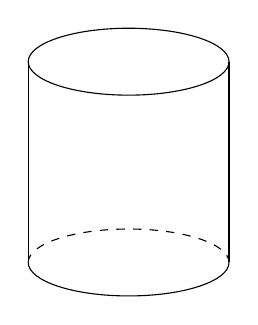
\begin{tikzpicture}[scale=0.85]
	%sichtbarer Teil der unteren Grundflaeche (vorderer Halbkreis)
	\draw (0,0.5) arc(-180:0:1.5cm and 0.5cm);
	%nicht sichtbarer Teil der unteren Grundflaeche (hinterer Halbkreis)
	\draw[dashed] (0,0.5) arc(180:0:1.5cm and 0.5cm);
	%linke Mantellinie
	\draw(0,0.5) -- (0,3.5);
	%obere Grundflaeche (vollstaendig sichtbar)
	\draw (0,3.5) arc(180:-180:1.5cm and 0.5cm);
	%rechte Mantellinie
	\draw (3,0.5) -- (3,3.5);
\end{tikzpicture}
\end{lstlisting}

\begin{lstlisting}[style=latex]
% Quader
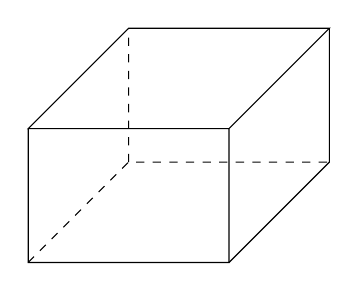
\begin{tikzpicture}[scale=0.85]
	%sichtbare Mantellinien
	\draw (0,2) -- (0,0) -- (3,0) -- (3,2) -- (0,2) -- (1.5,3.5) -- (4.5,3.5) -- (3,2);
	\draw (4.5,3.5) -- (4.5,1.5) -- (3,0);
	%nicht sichtbare Mantellinien
	\draw[dashed] (0,0) -- (1.5,1.5) -- (4.5,1.5) (1.5,1.5) -- (1.5,3.5);
\end{tikzpicture}
\end{lstlisting}

\begin{lstlisting}[style=latex]
% Dreiseitiges Prisma
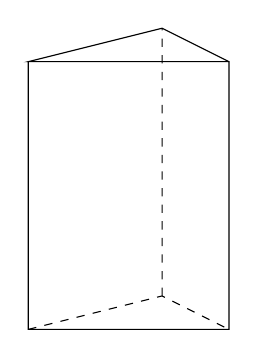
\begin{tikzpicture}[scale=0.85]
	%sichtbare Mantellinien
	\draw (0,4) -- (0,0) -- (3,0) -- (3,4) -- (0,4) -- (2,4.5) -- (3,4);
	%nicht sichtbare Mantellinien (hintere dreieckige Grundflaeche)
	\draw[dashed] (0,0) -- (2,0.5) -- (3,0) (2,0.5) -- (2,4.5);
\end{tikzpicture}
\end{lstlisting}

\begin{ausgabe}
	\begin{multicols}{3}
		% Zylinder
		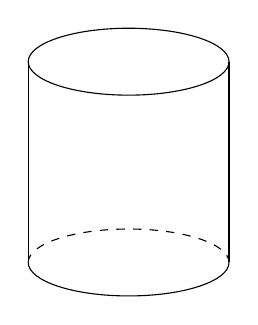
\begin{tikzpicture}[scale=0.85]
			  %sichtbarer Teil der unteren Grundflaeche (vorderer Halbkreis)
			  \draw (0,0.5) arc(-180:0:1.5cm and 0.5cm);
			  %nicht sichtbarer Teil der unteren Grundflaeche (hinterer Halbkreis)
			  \draw[dashed] (0,0.5) arc(180:0:1.5cm and 0.5cm);
			  %linke Mantellinie
			  \draw(0,0.5) -- (0,3.5);
			  %obere Grundflaeche (vollstaendig sichtbar)
			  \draw (0,3.5) arc(180:-180:1.5cm and 0.5cm);
			  %rechte Mantellinie
			  \draw (3,0.5) -- (3,3.5);
		\end{tikzpicture}
	
		% Quader (niedriger als Wuerfel)
		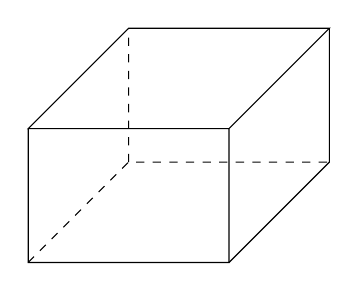
\begin{tikzpicture}[scale=0.85]
			  %sichtbare Mantellinien
			  \draw (0,2) -- (0,0) -- (3,0) -- (3,2) -- (0,2) -- (1.5,3.5) -- (4.5,3.5) -- (3,2);
			  \draw (4.5,3.5) -- (4.5,1.5) -- (3,0);
			  %nicht sichtbare Mantellinien
			  \draw[dashed] (0,0) -- (1.5,1.5) -- (4.5,1.5) (1.5,1.5) -- (1.5,3.5);
		\end{tikzpicture}
	
		% Dreiseitiges Prisma
		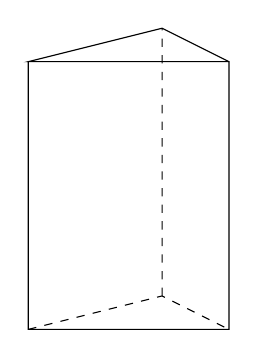
\begin{tikzpicture}[scale=0.85]
			  %sichtbare Mantellinien
			  \draw (0,4) -- (0,0) -- (3,0) -- (3,4) -- (0,4) -- (2,4.5) -- (3,4);
			  %nicht sichtbare Mantellinien (hintere dreieckige Grundflaeche)
			  \draw[dashed] (0,0) -- (2,0.5) -- (3,0) (2,0.5) -- (2,4.5);
		\end{tikzpicture}
	\end{multicols}
\end{ausgabe}

Die Darstellung dreidimensionaler Objekte erfolgt durch eine Kombination aus sichtbaren und unsichtbaren (gestrichelten) Linien. Der Befehl \texttt{arc} erzeugt Bögen, wobei die Parameter die Start- und Endwinkel sowie die Radien definieren. Der Parameter \texttt{scale} im Optionsbereich der \texttt{tikzpicture}-Umgebung skaliert die gesamte Zeichnung, was besonders bei komplexen Objekten nützlich ist.


%%%%  KAPITEL 2  %%%%
\section{Koordinaten definieren und Winkel zeichnen}

Ti\textit{k}Z bietet verschiedene Möglichkeiten, Koordinaten zu definieren und zu verwenden. Mit dem \texttt{\textbackslash coordinate}-Befehl können Sie benannte Punkte erstellen, die später referenziert werden können. Dies ist besonders hilfreich bei komplexen Zeichnungen, da es den Code übersichtlicher macht und Änderungen erleichtert.

\begin{lstlisting}[style=latex]
\begin{tikzpicture}
	%Koordinaten definieren
	\coordinate (A) at (0,0);
	\coordinate (B) at (6,0);
	\coordinate (C) at (2,2.7);
	%Dreieck zeichnen
	\draw (A) -- (B) -- (C) -- cycle; 
	%Bezeichnungen setzen
	\draw node at (3,-0.35) {Hypotenuse} node[rotate=-35] at (4.1,1.55) {Gegenkathete} node[rotate=53.5] at (0.8,1.55) {Ankathete};
	%Winkel zeichnen und beschriften
	\pic [draw,"\scriptsize{$\alpha$}",angle radius=0.65cm] {angle=B--A--C};
	\pic [draw,"\scriptsize{$\beta$}",angle radius=0.85cm] {angle=C--B--A};
	\pic [draw,"\scriptsize{$\cdot$}",angle radius=0.45cm] {angle=A--C--B};
\end{tikzpicture}
\end{lstlisting}

\begin{ausgabe}
	\begin{center}\begin{tikzpicture}
		%Koordinaten definieren
		\coordinate (A) at (0,0);
		\coordinate (B) at (6,0);
		\coordinate (C) at (2,2.7);
		%Dreieck zeichnen
		\draw (A) -- (B) -- (C) -- cycle; 
		%Bezeichnungen setzen
		\draw node at (3,-0.35) {Hypotenuse} node[rotate=-35] at (4.1,1.55) {Gegenkathete} node[rotate=53.5] at (0.8,1.55) {Ankathete};
		%Winkel zeichnen und beschriften
		\pic [draw,"\scriptsize{$\alpha$}",angle radius=0.65cm] {angle=B--A--C};
		\pic [draw,"\scriptsize{$\beta$}",angle radius=0.85cm] {angle=C--B--A};
		\pic [draw,"\scriptsize{$\cdot$}",angle radius=0.45cm] {angle=A--C--B};
	\end{tikzpicture}\end{center}
\end{ausgabe}

Im obigen Beispiel werden mehrere wichtige Techniken demonstriert:

\begin{itemize}
    \item \texttt{\textbackslash coordinate (Name) at (x,y)}: Definiert einen benannten Punkt an den Koordinaten \texttt{(x,y)}.
    \item \texttt{node at (x,y) \{Inhalt\}}: Platziert Text oder mathematische Ausdrücke an bestimmten Positionen.
    \item \texttt{\textbackslash pic}: Zeichnet spezielle Elemente wie Winkel zwischen drei Punkten.
    \item \texttt{rotate=Winkel}: Rotiert ein Element um den angegebenen Winkel.
\end{itemize}

Der \texttt{\textbackslash pic}-Befehl ist besonders nützlich für Winkeldarstellungen in geometrischen Figuren. Mit \texttt{angle=P1--P2--P3} wird der Winkel zwischen den Punkten P1, P2 und P3 dargestellt, wobei P2 der Scheitel ist. Der Parameter \texttt{angle radius} bestimmt die Größe des Winkelbogens.


%%%%  KAPITEL 3  %%%%
\section{Schleifen mit \texttt{\textbackslash foreach}}

Ti\textit{k}Z bietet mit dem \texttt{\textbackslash foreach}-Befehl eine leistungsstarke Möglichkeit, repetitive Elemente zu zeichnen, ohne den Code zu duplizieren. Dies ist besonders nützlich für Gitterstrukturen, regelmäßige Muster oder wenn mehrere ähnliche Elemente platziert werden sollen.

\begin{lstlisting}[style=latex]
%Quadrat mit vertikaler Aufteilung
\begin{tikzpicture}
	\draw (0,0) rectangle (4,4);
	\draw (2,0) -- (2,4);
\end{tikzpicture}
\end{lstlisting}

\begin{lstlisting}[style=latex]
%Quadrat mit horizontaler und vertikaler Aufteilung
\begin{tikzpicture}
	\draw (0,0) rectangle (4,4);
	\draw (2,0) -- (2,4);
	\draw (0,2) -- (4,2);
\end{tikzpicture}
\end{lstlisting}

\begin{lstlisting}[style=latex]
%Quadrat mit horizontaler und vertikaler Aufteilung durch Schleifen

\begin{tikzpicture}
	\draw (0,0) rectangle (4,4);
	\foreach \i in {1,2,3}{
		\draw (\i,0) -- (\i,4);
		\draw (0,\i) -- (4,\i);
	}
\end{tikzpicture}
\end{lstlisting}

\begin{ausgabe}
	\begin{multicols}{3}
		\begin{tikzpicture}
		 	\draw (0,0) rectangle (4,4);
		  	\draw (2,0) -- (2,4);
		\end{tikzpicture}
		\begin{tikzpicture}
	  		\draw (0,0) rectangle (4,4);
	  		\draw (2,0) -- (2,4);
	  		\draw (0,2) -- (4,2);	
		\end{tikzpicture}
		
\begin{tikzpicture}
	 		 \draw (0,0) rectangle (4,4);
	  		\foreach \i in {1,2,3}{
	   	 		\draw (\i,0) -- (\i,4);
	    			\draw (0,\i) -- (4,\i);
	  		}
		\end{tikzpicture}
	\end{multicols}
\end{ausgabe}

Die \texttt{foreach}-Schleife im dritten Beispiel zeichnet drei vertikale und drei horizontale Linien mit einem einzigen Befehlsblock. Die Variable \texttt{\textbackslash i} durchläuft die Werte 1, 2 und 3 und für jeden Wert werden die entsprechenden Linien gezeichnet. Dies macht den Code nicht nur kürzer, sondern auch übersichtlicher und leichter zu ändern.

Das Format \texttt{foreach \textbackslash i in \{Werte\}} kann verschiedene Wertebereiche annehmen:
\begin{itemize}
	\item Diskrete Werte: \texttt{\{1,2,3\}}
    	\item Bereiche mit Schrittweite: \texttt{\{0,0.5,...,4\}} (von 0 bis 4 in 0.5er-Schritten)
    	\item Winkelwerte: \texttt{\{0,45,...,315\}} (von 0 bis 315 in 45°-Schritten)
\end{itemize}


%%%%  KAPITEL 4  %%%%
\section{Flächen füllen mit \texttt{\textbackslash fill}}

Ti\textit{k}Z erlaubt nicht nur das Zeichnen von Linien, sondern auch das Färben von Flächen. Der Befehl \texttt{\textbackslash fill} füllt geschlossene Bereiche mit einer angegebenen Farbe.

\begin{lstlisting}[style=latex]
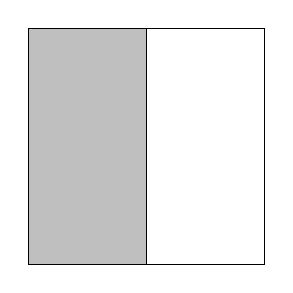
\begin{tikzpicture}[scale=0.75]
	%Fuellung einer vorgegebenen Form
	\fill[gray, opacity=0.5] (0,0) rectangle (2,4);
	\draw (0,0) rectangle (4,4);
	\draw (2,0) -- (2,4);
\end{tikzpicture}
\end{lstlisting}
\begin{lstlisting}[style=latex]
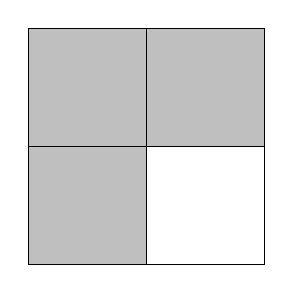
\begin{tikzpicture}[scale=0.75]
	%Fuellung entlange eines Pfades
	\fill[gray, opacity=0.5] (0,0) -- (2,0) -- (2,2) -- (4,2) -- (4,4) -- (0,4) -- cycle;
	\draw (0,0) rectangle (4,4);
	\draw (2,0) -- (2,4);
	\draw (0,2) -- (4,2);
\end{tikzpicture}
\end{lstlisting}

\begin{lstlisting}[style=latex]
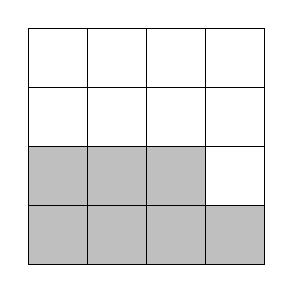
\begin{tikzpicture}[scale=0.75]
	%Fuellung entlang eines Pfades
	\fill[gray, opacity=0.5] (0,0) -- (4,0) -- (4,1) -- (3,1) -- (3,2) -- (0,2) -- cycle;
	\draw (0,0) rectangle (4,4);
	\foreach \i in {1,2,3}{
		\draw (\i,0) -- (\i,4);
		\draw (0,\i) -- (4,\i);
	}
\end{tikzpicture}
\end{lstlisting}

\begin{ausgabe}
	\begin{multicols}{3}
		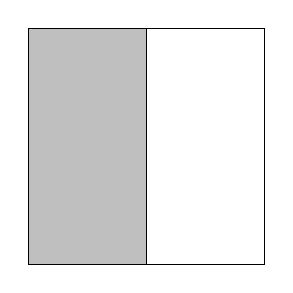
\begin{tikzpicture}[scale=0.75]
			  \fill[gray, opacity=0.5] (0,0) rectangle (2,4);
			  \draw (0,0) rectangle (4,4);
			  \draw (2,0) -- (2,4);
		\end{tikzpicture}

		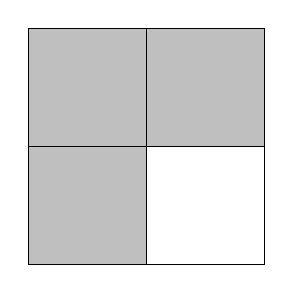
\begin{tikzpicture}[scale=0.75]
			  \fill[gray, opacity=0.5] (0,0) -- (2,0) -- (2,2) -- (4,2) -- (4,4) -- (0,4) -- cycle;
			  \draw (0,0) rectangle (4,4);
			  \draw (2,0) -- (2,4);
			  \draw (0,2) -- (4,2);
		\end{tikzpicture}

		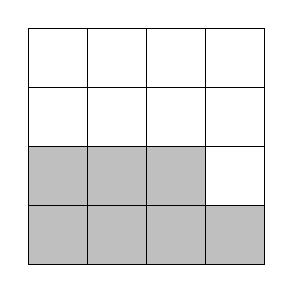
\begin{tikzpicture}[scale=0.75]
			  \fill[gray, opacity=0.5] (0,0) -- (4,0) -- (4,1) -- (3,1) -- (3,2) -- (0,2) -- cycle;
			  \draw (0,0) rectangle (4,4);
			  \foreach \i in {1,2,3}{
				    \draw (\i,0) -- (\i,4);
				    \draw (0,\i) -- (4,\i);
			  }
		\end{tikzpicture}
	\end{multicols}
\end{ausgabe}


Der Befehl \texttt{\textbackslash fill} funktioniert ähnlich wie \texttt{\textbackslash draw}, erfordert jedoch einen geschlossenen Pfad. Durch die Option \texttt{opacity=0.5} lässt sich die Füllung halbtransparent gestalten, was besonders bei überlappenden Elementen vorteilhaft ist. Das Schlüsselwort \texttt{cycle} am Ende eines Pfads ist äußerst nützlich, da es diesen automatisch schließt, indem es eine Linie zum Startpunkt zurückzieht, ohne dass der Pfad manuell geschlossen werden muss. Neben den separaten Befehlen \texttt{\textbackslash fill} und \texttt{\textbackslash draw} steht auch \texttt{\textbackslash filldraw} zur Verfügung, das beides in einem einzigen Befehl kombiniert und somit den Code übersichtlicher gestaltet.

Die Farben können vielfältig sein:
\begin{itemize}
    \item Standardfarben: \texttt{red, green, blue, cyan, magenta, yellow, black, white}
    \item Abgemischte Farben: \texttt{red!30!blue} (30\% Rot, 70\% Blau)
    \item Transparenz: \texttt{opacity=0.5} (50\% transparent)
\end{itemize}


%%%%  KAPITEL 5  %%%%
\section{Koordinatenberechnungen mit der \texttt{calc}-Bibliothek}

Die \texttt{calc}-Bibliothek erlaubt es, Koordinaten direkt in Ti\textit{k}Z-Befehlen zu berechnen. Dies ist besonders nützlich für dynamische Zeichnungen oder wenn Punkte von anderen abgeleitet werden sollen. Dabei dient das \texttt{\$}-Symbol, wie bei einer mathematischen Umgebung dazu, \hologo{LaTeX} zu signalisieren, dass hier gerechnet wird. Wichtig ist, dass innerhalb des Ausdrucks \texttt{(\$ ... \$)} auch wieder ein zweidimensionaler Vektor errechnet wird. Ansonsten bekommt man an dieser Stelle eine Fehlermeldung.

\begin{lstlisting}[style=latex]
%Kreis mit 6 Segmenten
\begin{tikzpicture}[scale=0.9]
	\draw (2,2) circle (2cm);
	%Linien die vom Mittelpunkt wegfuehren
	\foreach \i in {0,60,...,300} {
		\draw (2,2) -- ($(2,2) + cos(\i)*(2,0) +sin(\i)*(0,2)$);		%trigonometrische Berechnungen
	}
\end{tikzpicture}
\end{lstlisting}

\begin{lstlisting}[style=latex]
%Kreis mit 5 Segmenten
\begin{tikzpicture}[scale=0.9]
	\draw (2,2) circle (2cm);
	%Linien die vom Mittelpunkt wegfuehren
	\foreach \i in {0,72,144,216,288} {
		\draw (2,2) -- ($(2,2) + cos(\i)*(2,0) +sin(\i)*(0,2)$);		%trigonometrische Berechnungen
	}
\end{tikzpicture}
\end{lstlisting}

\begin{lstlisting}[style=latex]
%Gleichseitiges Dreieck mit 6 Segmenten
\begin{tikzpicture}[scale=0.9]
	%Dreieck zeichnen
	\draw (0,0) -- (4,0) -- ($(2,0) +sqrt(12)*(0,1)$) -- cycle;
	%Mittelsenkrechten zeichnen durch Berechnungen mit dem Satz des Pythagoras
	\draw (2,0) -- ($(2,0) +sqrt(12)*(0,1)$);
	\draw (0,0) -- ($(3,0) +sqrt(3)*(0,1)$);
	\draw (4,0) -- ($(1,0) +sqrt(3)*(0,1)$);
\end{tikzpicture}
\end{lstlisting}

\begin{lstlisting}[style=latex]
%Regelmaessiges Acht-Eck
\begin{tikzpicture}[scale=0.9]
	%Schleifenzeichnung vom Mittelpunkt ausgehend mit Hilfe trigonometrischer Berechnungen
	\foreach \i in {0,45,...,315} {
		\draw (2,2) -- ($(2,2) + cos(\i)*(2,0) + sin(\i)*(0,2)$) -- ($(2,2) + cos(\i +45)*(2,0) +sin(\i +45)*(0,2)$);
	}
\end{tikzpicture}
\end{lstlisting}

\begin{ausgabe}
	\begin{multicols}{4}
		\begin{tikzpicture}[scale=0.9]
			  \draw (2,2) circle (2cm);
			  \foreach \i in {0,60,...,300} {
				    \draw (2,2) -- ($(2,2) + cos(\i)*(2,0) +sin(\i)*(0,2)$);
			  }
		\end{tikzpicture}
	
		\begin{tikzpicture}[scale=0.9]
			  \draw (2,2) circle (2cm);
			  \foreach \i in {0,72,144,216,288} {
				    \draw (2,2) -- ($(2,2) + cos(\i)*(2,0) +sin(\i)*(0,2)$);
			  }
		\end{tikzpicture}
	
		\begin{tikzpicture}[scale=0.9]
			  \draw (0,0) -- (4,0) -- ($(2,0) +sqrt(12)*(0,1)$) -- cycle;
			  \draw (2,0) -- ($(2,0) +sqrt(12)*(0,1)$);
			  \draw (0,0) -- ($(3,0) +sqrt(3)*(0,1)$);
			  \draw (4,0) -- ($(1,0) +sqrt(3)*(0,1)$);
		\end{tikzpicture}
	
		\begin{tikzpicture}[scale=0.9]
			  \foreach \i in {0,45,...,315} {
				    \draw (2,2) -- ($(2,2) + cos(\i)*(2,0) + sin(\i)*(0,2)$) -- ($(2,2) + cos(\i +45)*(2,0) +sin(\i +45)*(0,2)$);
			  }
		\end{tikzpicture}
	\end{multicols}
\end{ausgabe}

Die \texttt{calc}-Bibliothek ermöglicht komplexe Koordinatenberechnungen direkt innerhalb der Ti\textit{k}Z-Befehle. Im Ausdruck \texttt{\$(2,2) + cos(\textbackslash i)*(2,0) +sin(\textbackslash i)*(0,2)\$} wird zunächst ein Basispunkt \texttt{(2,2)} definiert, dann der Kosinus des Winkels \texttt{\textbackslash i} mit dem Vektor \texttt{(2,0)} multipliziert sowie der Sinus des Winkels \texttt{\textbackslash i} mit dem Vektor \texttt{(0,2)} multipliziert und schließlich werden alle Vektoren addiert, um die resultierende Koordinate zu erhalten. Diese Technik ist besonders nützlich für die Erstellung regelmäßiger Polygone, die Platzierung von Punkten auf Kreisen oder Ellipsen, die Berechnung geometrischer Konstruktionen sowie die dynamische Anpassung von Zeichnungen basierend auf Parametern. Zusätzlich stehen verschiedene mathematische Funktionen wie \texttt{sqrt} (Wurzel), \texttt{abs} (Betrag), \texttt{sin} und \texttt{cos} zur Verfügung, die die Berechnungsmöglichkeiten erweitern.


%%%% KAPITEL 6  %%%%
\section{Füllen entlang berechneter Pfade}

Die \texttt{calc}-Bibliothek kann auch hervorragend mit dem \texttt{\textbackslash fill}-Befehl kombiniert werden, um komplexe gefüllte Bereiche zu erzeugen. Diese Technik ist besonders nützlich für die Darstellung von Kreissektoren, Flächen unter Kurven und anderen mathematischen Formen.

\begin{lstlisting}[style=latex]
% Kreissektor von 0 Grad bis 300 Grad fuellen
\begin{tikzpicture}[scale=0.75]
	\fill[gray, opacity=0.5] (2,2) -- 							% Vom Mittelpunkt starten
			($(2,2) + cos(0)*(2,0) +sin(0)*(0,2)$) 			% Zum Startpunkt des Bogens (0 Grad)
			arc (0:300:2) 															% Bogen von 0 Grad bis 300 Grad mit Radius 2
			($(2,2) + cos(300)*(2,0) +sin(300)*(0,2)$) 	% Endpunkt des Bogens
			-- cycle;																		% Zurueck zum Mittelpunkt schliessen
	\draw (2,2) circle (2cm);
	\foreach \i in {0,60,...,300} {
		\draw (2,2) -- ($(2,2) + cos(\i)*(2,0) +sin(\i)*(0,2)$);
	}
\end{tikzpicture}
\end{lstlisting}

\begin{lstlisting}[style=latex]
% Teilflaeche des Dreiecks fuellen
\begin{tikzpicture}[scale=0.75]
	\fill[gray, opacity=0.5] (0,0) --   	%Linke untere Ecke
			(2,0) -- 													%Mittelpunkt das Basis
			($(2,0) +sqrt(12)*(0,0.333)$) 		%Punkt bei 1/3 der Hoehe ueber der Mitte
			(4,0) -- 													% Rechte untere Ecke
			($(2,0) +sqrt(12)*(0,1)$) -- 			%Spitze des Dreiecks
			cycle;  													%Pfad schliessen.
	\draw (0,0) -- (4,0) -- ($(2,0) +sqrt(12)*(0,1)$) -- cycle;
	\draw (2,0) -- ($(2,0) +sqrt(12)*(0,1)$);
	\draw (0,0) -- ($(3,0) +sqrt(3)*(0,1)$);
	\draw (4,0) -- ($(1,0) +sqrt(3)*(0,1)$);
\end{tikzpicture}
\end{lstlisting}

\begin{lstlisting}[style=latex]
%Acht-Eck segmentweise fuellen
\begin{tikzpicture}[scale=0.75]
	\foreach \i in {0,45,...,180}{
		\fill[gray, opacity=0.5] (2,2) -- 												%Vom Mittelpunkt starten
				($(2,2) + cos(\i)*(2,0) + sin(\i)*(0,2)$) -- 					%Erster Eckpunkt
				($(2,2) + cos(\i +45)*(2,0) +sin(\i +45)*(0,2)$) --  	%Zweiter Eckpunkt
				cycle;   																							%Pfad schliessen
	}
	\foreach \i in {0,45,...,315} {
		\draw (2,2) -- ($(2,2) + cos(\i)*(2,0) + sin(\i)*(0,2)$) -- ($(2,2) + cos(\i +45)*(2,0) +sin(\i +45)*(0,2)$);
	}
\end{tikzpicture}
\end{lstlisting}


\begin{ausgabe}
	\begin{multicols}{3}
		% Kreissektor von 0 Grad bis 300 Grad fuellen
		\begin{tikzpicture}[scale=0.75]
			\fill[gray, opacity=0.5] (2,2) -- 							% Vom Mittelpunkt starten
					($(2,2) + cos(0)*(2,0) +sin(0)*(0,2)$) 			% Zum Startpunkt des Bogens (0 Grad)
					arc (0:300:2) 															% Bogen von 0 Grad bis 300 Grad mit Radius 2
					($(2,2) + cos(300)*(2,0) +sin(300)*(0,2)$) 	% Endpunkt des Bogens
					-- cycle;																		% Zurueck zum Mittelpunkt schliessen
			\draw (2,2) circle (2cm);
			% Segmentlinien vom Mittelpunkt zu den Teilungspunkten zeichnen
			\foreach \i in {0,60,...,300} {
				\draw (2,2) -- ($(2,2) + cos(\i)*(2,0) +sin(\i)*(0,2)$);
			}
		\end{tikzpicture}
	
		% Teilflaeche des Dreiecks fuellen
		\begin{tikzpicture}[scale=0.75]
			\fill[gray, opacity=0.5] (0,0) --   %Linke untere Ecke
					(2,0) -- 			%Mittelpunkt das Basis
					($(2,0) +sqrt(12)*(0,0.333)$) 		%Punkt bei 1/3 der Höehe ueber der Mitte
					(4,0) -- % Rechte untere Ecke
					($(2,0) +sqrt(12)*(0,1)$) -- cycle; %Spitze des Dreiecks und Pfad schließen.
			%Dreieck zeichnen
			\draw (0,0) -- (4,0) -- ($(2,0) +sqrt(12)*(0,1)$) -- cycle;
			%Mittelsenkrechte zeichnen
			\draw (2,0) -- ($(2,0) +sqrt(12)*(0,1)$);
			\draw (0,0) -- ($(3,0) +sqrt(3)*(0,1)$);
			\draw (4,0) -- ($(1,0) +sqrt(3)*(0,1)$);
		\end{tikzpicture}
	
		%Acht-Eck segmentweise fuellen
		\begin{tikzpicture}[scale=0.75]
			\foreach \i in {0,45,...,180}{
				\fill[gray, opacity=0.5] (2,2) -- 												%Vom Mittelpunkt starten
						($(2,2) + cos(\i)*(2,0) + sin(\i)*(0,2)$) -- 					%Erster Eckpunkt
						($(2,2) + cos(\i +45)*(2,0) +sin(\i +45)*(0,2)$) --  	%Zweiter Eckpunkt
						cycle;   																							%Pfad schliessen
			}
			\foreach \i in {0,45,...,315} {
				\draw (2,2) -- ($(2,2) + cos(\i)*(2,0) + sin(\i)*(0,2)$) -- ($(2,2) + cos(\i +45)*(2,0) +sin(\i +45)*(0,2)$);
			}
		\end{tikzpicture}
	\end{multicols}
\end{ausgabe}

In den obigen Beispielen werden Kreissektoren und komplexe polygonale Bereiche gefüllt. Besonders hervorzuheben ist die Kombination von:
\begin{itemize}
	\item \texttt{\textbackslash fill}-Befehl für die Flächenfüllung
	\item \texttt{arc} für Kreisbögen
	\item \texttt{\textbackslash foreach}-Befehl für Schleifen mit wiederholtem Muster
	\item \texttt{calc}-Bibliothek für präzise Koordinatenberechnung zwischen den \texttt{\$}-Symbolen
\end{itemize}

Im ersten Beispiel wird ein Kreissektor von 0° bis 300° gefüllt, indem zunächst vom Mittelpunkt zum Startpunkt des Bogens eine Linie gezeichnet wird, dann der Bogen selbst und schließlich zurück zum Mittelpunkt. Das Schlüsselwort \texttt{cycle} ist hier entscheidend, um den Pfad zu schließen.

Die Kombination dieser Techniken erlaubt die Erstellung komplexer mathematischer Visualisierungen, die für den MINT-Unterricht besonders wertvoll sind.


%%%%  KAPITEL 7  %%%%
\section{Kästchenpapier mit \texttt{multicols} und der \texttt{topline}-Option}

Für Arbeitsblätter ist oft ein Kästchenpapier-Hintergrund nützlich, auf dem Schülerinnen und Schüler zeichnen oder konstruieren können. Mit Ti\textit{k}Z lässt sich solches Papier leicht erstellen und in Dokumente einbetten.

\begin{lstlisting}[style=latex]
\begin{multicols}{2}											%Zweispaltiges Layout fuer platzsparende Anordnung
	\begin{enumerate}[(a)]									%Nummerierung mit Kleinbuchstaben: (a), (b), (c), ...
		\item \begin{tikzpicture}[topline]   	%Erste Aufgabe mit topline-Ausrichtung
			%Vertikale Gitternetzlinien zeichnen
			\foreach \i in {1,1.5,...,7} {
				\draw[gray, very thin] (\i,-0.25) -- (\i,4.75);
			}
			%Horizontale Gitternetzlinien zeichnen
			\foreach \i in {0,0.5,...,4.5} {
				\draw[gray, very thin] (0.75,\i) -- (7.25,\i);
			}
		\end{tikzpicture}

		\item \begin{tikzpicture}[topline]
			\foreach \i in {9.5,10,...,15} {
				\draw[gray, very thin] (\i,-0.25) -- (\i,4.75);
			}
			\foreach \i in {0,0.5,...,4.5} {
				\draw[gray, very thin] (9.25,\i) -- (15.25,\i);
			}
		\end{tikzpicture}
	\end{enumerate}
\end{multicols}
\end{lstlisting}

\begin{ausgabe}
	\begin{multicols}{2}											%Zweispaltiges Layout fuer platzsparende Anordnung
		\begin{enumerate}[(a)]									%Nummerierung mit Kleinbuchstaben: (a), (b), (c), ...
			\item \begin{tikzpicture}[topline]   	%Erste Aufgabe mit topline-Ausrichtung
				%Vertikale Gitternetzlinien zeichnen
				\foreach \i in {1,1.5,...,7} {
					\draw[gray, very thin] (\i,-0.25) -- (\i,4.75);
				}
				%Horizontale Gitternetzlinien zeichnen
				\foreach \i in {0,0.5,...,4.5} {
					\draw[gray, very thin] (0.75,\i) -- (7.25,\i);
				}
			\end{tikzpicture}
	
			\item \begin{tikzpicture}[topline]
				\foreach \i in {9.5,10,...,15} {
					\draw[gray, very thin] (\i,-0.25) -- (\i,4.75);
				}
				\foreach \i in {0,0.5,...,4.5} {
					\draw[gray, very thin] (9.25,\i) -- (15.25,\i);
				}
			\end{tikzpicture}
		\end{enumerate}
	\end{multicols}
\end{ausgabe}

In diesem Beispiel werden mehrere wichtige Techniken für Arbeitsblätter demonstriert. Das Paket \texttt{multicols} wird verwendet, um die Aufgaben platzsparend in zwei Spalten anzuordnen, während die \texttt{enumerate}-Umgebung mit der Option \texttt{[(a)]} die Aufgaben übersichtlich mit Kleinbuchstaben nummeriert. Der in \texttt{newcommands.tex} definierte Stil \texttt{topline} sorgt dafür, dass die Ti\textit{k}Z-Zeichnungen bündig am oberen Rand der Aufzählung ausgerichtet werden, was ein konsistentes Erscheinungsbild gewährleistet. Mit \texttt{\textbackslash foreach}-Schleifen werden die Gitternetzlinien effizient erzeugt, ohne jeden einzelnen Strich manuell definieren zu müssen. Die Gitternetzlinien werden absichtlich etwas über den eigentlichen Zeichenbereich hinausgeführt – eine in Schulbüchern und Arbeitsblättern übliche Praxis.


%%%%  KAPITEL 8  %%%%
\section{Funktionen zeichnen mit \texttt{plot} und der \texttt{scope}-Umgebung}

Ti\textit{k}Z bietet leistungsstarke Möglichkeiten zum Plotten von Funktionen. Mit dem \texttt{plot}-Befehl können mathematische Funktionen direkt gezeichnet werden und die \texttt{\textbackslash clip}-Anweisung sorgt dafür, dass die Grafik auf den gewünschten Bereich beschränkt bleibt.

\begin{lstlisting}[style=latex]
\begin{tikzpicture}[topline, scale=0.5]		% topline-Ausrichtung
	% Gitternetzlinien zeichnen (sowohl vertikal als auch horizontal)
	\foreach \i in {-5,-4.5,...,5.5}{
		\draw[very thin, gray] (\i,-5.25) -- (\i,5.75);
		\draw[very thin, gray] (-5.25,\i) -- (5.75,\i);
	}
	% Koordinatenachsen mit Pfeilen zeichnen
	\draw[->, thick] (-5,0) -- (5.5,0) node[below] {\scriptsize{$x$}};
	\draw[->, thick] (0,-5) -- (0,5.5) node[left] {\scriptsize{$y$}};
	\foreach \i in {-5,-4,-3,-2,-1,1,2,3,4,5}{
		\draw[thick] (\i,0.1) -- (\i,-0.1);
		\draw[thick] (0.1,\i) -- (-0.1,\i);
	}
	%Achseneinteilung
	\draw node[below] at (1,0) {\tiny{$1$}} node[left] at (0,1) {\tiny{$1$}};
	% scope-Umgebung fuer kontrollierte Funktionsdarstellung 
	\begin{scope}
		\clip (-5.25,-5.25) rectangle (5.75,5.75);
		\draw[thick] plot[domain=0:5.75] (\x,{(\x-3)^2}) node at (4.5,5) {\scriptsize{$f(x)$}};
		\draw[thick] plot[domain=-3:1] (\x,{(\x+1)^2+3}) node at (-3.25,5) {\scriptsize{$g(x)$}};
		\draw[thick] plot[domain=-5.25:1.5] (\x,{(\x+2)^2-4}) node at (-3.25,-4.25) {\scriptsize{$h(x)$}};
	\end{scope}
\end{tikzpicture}
\end{lstlisting}


\begin{ausgabe}
	\begin{center}\begin{tikzpicture}[topline, scale=0.5]		% topline-Ausrichtung
		% Gitternetzlinien zeichnen (sowohl vertikal als auch horizontal)
		\foreach \i in {-5,-4.5,...,5.5}{
			\draw[very thin, gray] (\i,-5.25) -- (\i,5.75);
			\draw[very thin, gray] (-5.25,\i) -- (5.75,\i);
		}
		% Koordinatenachsen mit Pfeilen zeichnen
		\draw[->, thick] (-5,0) -- (5.5,0) node[below] {\scriptsize{$x$}};
		\draw[->, thick] (0,-5) -- (0,5.5) node[left] {\scriptsize{$y$}};
		\foreach \i in {-5,-4,-3,-2,-1,1,2,3,4,5}{
			\draw[thick] (\i,0.1) -- (\i,-0.1);
			\draw[thick] (0.1,\i) -- (-0.1,\i);
		}
		%Achseneinteilung
		\draw node[below] at (1,0) {\tiny{$1$}} node[left] at (0,1) {\tiny{$1$}};
		% scope-Umgebung fuer kontrollierte Funktionsdarstellung 
		\begin{scope}
			\clip (-5.25,-5.25) rectangle (5.75,5.75);
			\draw[thick] plot[domain=0:5.75] (\x,{(\x-3)^2}) node at (4.5,5) {\scriptsize{$f(x)$}};
			\draw[thick] plot[domain=-3:1] (\x,{(\x+1)^2+3}) node at (-3.25,5) {\scriptsize{$g(x)$}};
			\draw[thick] plot[domain=-5.25:1.5] (\x,{(\x+2)^2-4}) node at (-3.25,-4.25) {\scriptsize{$h(x)$}};
		\end{scope}
	\end{tikzpicture}\end{center}
\end{ausgabe}

Bei der Darstellung von Funktionsgraphen sind mehrere Techniken von zentraler Bedeutung. Die \texttt{scope}-Umgebung erzeugt einen abgeschlossenen Bereich, in dem Befehle wie \texttt{\textbackslash draw} oder \texttt{plot} nur lokal wirken, ohne den Rest der Zeichnung zu beeinflussen. Die \texttt{\textbackslash clip}-Anweisung beschränkt dabei alle nachfolgenden Zeichnungen auf den angegebenen Bereich, in diesem Fall ein Rechteck um das Koordinatensystem. Der \texttt{plot[domain=a:b]}-Befehl zeichnet eine Funktion im angegebenen Intervall [a,b], wobei die Variable \texttt{\textbackslash x} dieses Intervall durchläuft und für jeden Wert der zugehörige Funktionswert berechnet wird. Für das Koordinatensystem selbst werden mit \texttt{\textbackslash foreach}-Schleifen die Gitternetzlinien und die Achseneinteilungen effizient erzeugt, während die Pfeile an den Achsenenden durch die Option \texttt{[->]} die Richtung verdeutlichen. Die Kombination von der \texttt{scope}-Umgebung zusammen mit dem durch \texttt{\textbackslash clip} eingeschränktem Bereich und dem \texttt{plot}-Befehl ist besonders wichtig, da viele Funktionen (wie z.B. $y = \frac{1}{x}$) außerhalb des sichtbaren Bereichs sehr große Werte annehmen können, was zu unerwünschten grafischen Artefakten führen würde, wenn man es nicht durch \texttt{\textbackslash clip} begrenzt.\\

Bei trigonometrischen Funktionen ist zu beachten, dass Ti\textit{k}Z standardmäßig mit Gradmaß arbeitet. Um Werte im Bogenmaß zu verwenden, wird das Suffix \texttt{r} an den Winkel angehängt.

\begin{lstlisting}[style=latex]
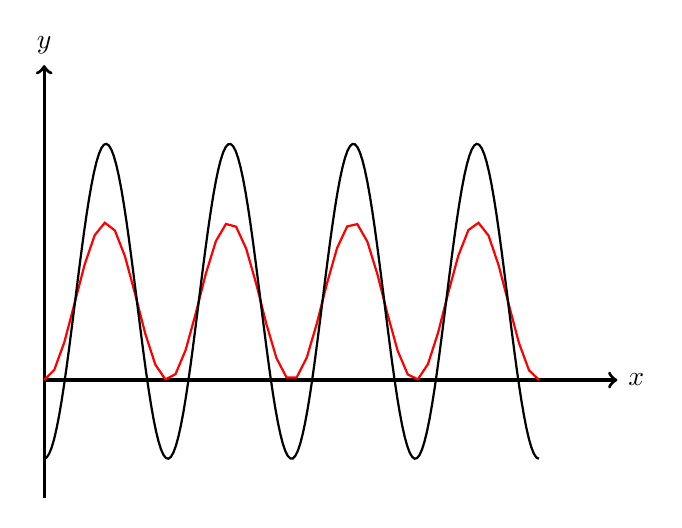
\begin{tikzpicture}
	%Koordinatenachsen zeichnen
	\draw[->, very thick] (0,0) -- (7.28,0) node[right] {$x$};
	\draw[->, very thick] (0,-1.5) -- (0,4) node[above] {$y$};
	%Funktionsplots
	\draw[thick, red, domain=0:6.285, samples=50] plot (\x,{sin((4*\x -1.57) r)+1});
	\draw[thick, domain=0:6.285, samples=200] plot (\x,{2*sin((4*\x -1.57) r)+1});
\end{tikzpicture}
\end{lstlisting}

\begin{ausgabe}
	\begin{center}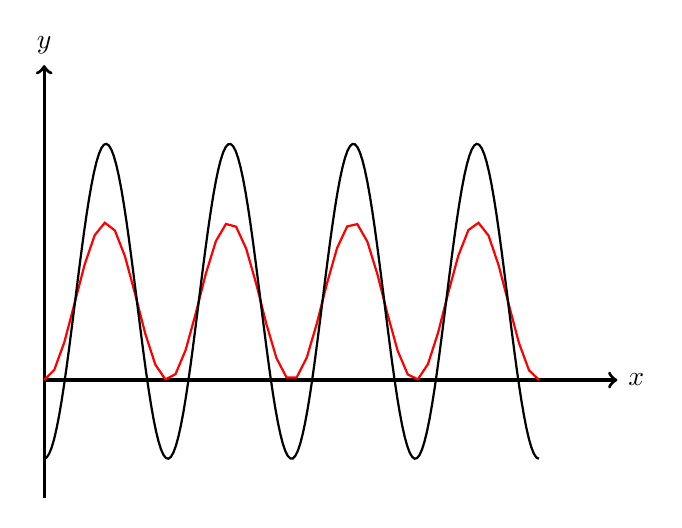
\begin{tikzpicture}
		%Koordinatenachsen zeichnen
		\draw[->, very thick] (0,0) -- (7.28,0) node[right] {$x$};
		\draw[->, very thick] (0,-1.5) -- (0,4) node[above] {$y$};
		%Funktionsplots
		\draw[thick, red, domain=0:6.285, samples=50] plot (\x,{sin((4*\x -1.57) r)+1});
		\draw[thick, domain=0:6.285, samples=200] plot (\x,{2*sin((4*\x -1.57) r)+1});
	\end{tikzpicture}\end{center}
\end{ausgabe}

In diesem Beispiel wird eine Sinuskurve mit gedämpfter Amplitude gezeichnet. Das Suffix \texttt{r} in der Notation \texttt{(4*\textbackslash x -0.85) r} ist besonders wichtig, da es den Ausdruck ins Bogenmaß umwandelt, wodurch Ti\textit{k}Z die trigonometrischen Funktionen korrekt berechnen kann. Der Parameter \texttt{samples=200} erhöht die Genauigkeit der Kurve deutlich, was besonders bei oszillierenden Funktionen wie Sinus und Kosinus wichtig ist, um unerwünschte Kantigkeit zu vermeiden. Die Funktion selbst wird nur in einem präzise definierten \texttt{domain}-Bereich gezeichnet, in diesem Fall von 0.25 bis 3.15 (ungefähr $\pi$), was ermöglicht, gezielt nur den relevanten Teil der Kurve darzustellen.


%%%%  KAPITEL 9  %%%%
\section{Flächen unter Funktionsgraphen füllen}

Eine häufige Anforderung im Mathematikunterricht ist die Darstellung von Flächen unter Funktionsgraphen, etwa für die Integralrechnung. Die Kombination von \texttt{scope}-Umgebung, \texttt{plot} und dem \texttt{\textbackslash fill}-Befehl ermöglicht präzise und ansprechende Visualisierungen.

\begin{lstlisting}[style=latex]
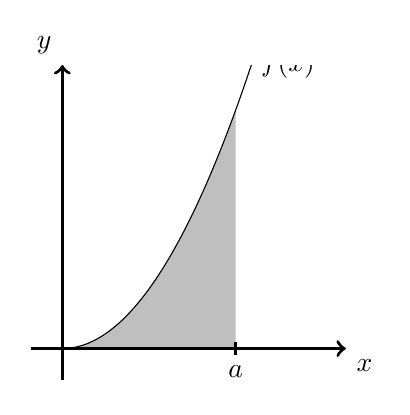
\begin{tikzpicture}[scale=0.8]
	\begin{scope}
		%Clip-Bereich
		\clip (-0.5,-0.5) rectangle (4.5,4.5);
		%Flaechenfuellung
		\fill[gray, opacity=0.5] (0,0) -- (2.75,0)  -- plot[smooth, domain=2.75:0] (\x,{0.5*\x*\x}) -- cycle;
		%Funktionsplot
		\draw plot[smooth, domain=0:3] (\x,{0.5*\x*\x}) node[right] {$f(x)$};
	\end{scope}
	%Koordinatenachsen und Beschriftungen
	\draw[->, very thick] (-0.5,0) -- (4.5,0) node[below right] {$x$};
	\draw[->, very thick] (0,-0.5) -- (0,4.5) node[above left] {$y$};
	\draw[very thick] (2.75,0.1) -- (2.75,-0.1) node[below] {$a$};
\end{tikzpicture}
\end{lstlisting}

\begin{lstlisting}[style=latex]
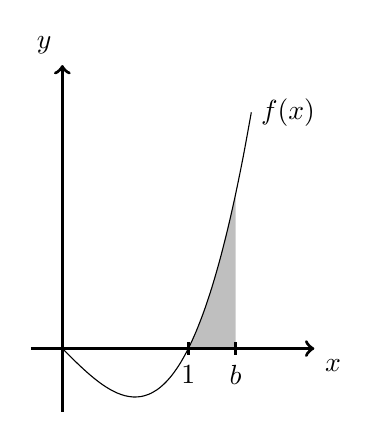
\begin{tikzpicture}[scale=0.8]
	\begin{scope}
		%Clip-Bereich
		\clip (-0.5,-1) rectangle (4.5,4.5);
		%Flaechenfuellung
		\fill[gray, opacity=0.5] (2,0) -- (2.75,0)  -- plot[smooth, domain=2.75:2] (\x,{0.5*(0.5*\x*\x*\x-2*\x)}) -- cycle;
		%Funktionsplot
		\draw plot[smooth, domain=0:3] (\x,{0.5*(0.5*\x*\x*\x-2*\x)}) node[right] {$f(x)$};
	\end{scope}
	%Koordinatenachsen und Beschriftungen
	\draw[->, very thick] (-0.5,0) -- (4,0) node[below right] {$x$};
	\draw[->, very thick] (0,-1) -- (0,4.5) node[above left] {$y$};
	\draw[very thick] (2,0.1) -- (2,-0.1) node[below] {$1$} (2.75,0.1) -- (2.75,-0.1) node[below] {$b$};
\end{tikzpicture}
\end{lstlisting}

\begin{lstlisting}[style=latex]
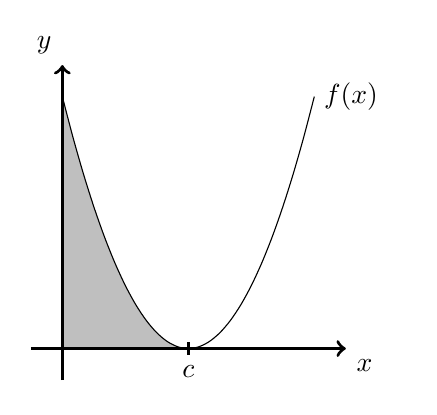
\begin{tikzpicture}[scale=0.8]
	\begin{scope}
		%Clip-Bereich
		\clip (0,0) rectangle (5.5,5);
		%Flaechenfuellung
		\fill[gray, opacity=0.5] (0,0) -- (2,0)  -- plot[smooth, domain=2:0] (\x,{(\x-2)*(\x-2)}) -- cycle;
		%Funktionsplot
		\draw plot[smooth, domain=0:4] (\x,{(\x-2)*(\x-2)}) node[right] {$f(x)$};
	\end{scope}
	%Koordinatenachsen und Beschriftungen
	\draw[->, very thick] (-0.5,0) -- (4.5,0) node[below right] {$x$};
	\draw[->, very thick] (0,-0.5) -- (0,4.5) node[above left] {$y$};
	\draw[very thick] (2,0.1) -- (2,-0.1) node[below] {$c$};
\end{tikzpicture}
\end{lstlisting}

\begin{ausgabe}
	\begin{multicols}{3}
		\begin{tikzpicture}[scale=0.8]
			\begin{scope}
				%Clip-Bereich
				\clip (-0.5,-0.5) rectangle (4.5,4.5);
				%Flaechenfuellung
				\fill[gray, opacity=0.5] (0,0) -- (2.75,0)  -- plot[smooth, domain=2.75:0] (\x,{0.5*\x*\x}) -- cycle;
				%Funktionsplot
				\draw plot[smooth, domain=0:3] (\x,{0.5*\x*\x}) node[right] {$f(x)$};
			\end{scope}
			%Koordinatenachsen und Beschriftungen
			\draw[->, very thick] (-0.5,0) -- (4.5,0) node[below right] {$x$};
			\draw[->, very thick] (0,-0.5) -- (0,4.5) node[above left] {$y$};
			\draw[very thick] (2.75,0.1) -- (2.75,-0.1) node[below] {$a$};
		\end{tikzpicture}
	
		\begin{tikzpicture}[scale=0.8]
			\begin{scope}
				%Clip-Bereich
				\clip (-0.5,-1) rectangle (4.5,4.5);
				%Flaechenfuellung
				\fill[gray, opacity=0.5] (2,0) -- (2.75,0)  -- plot[smooth, domain=2.75:2] (\x,{0.5*(0.5*\x*\x*\x-2*\x)}) -- cycle;
				%Funktionsplot
				\draw plot[smooth, domain=0:3] (\x,{0.5*(0.5*\x*\x*\x-2*\x)}) node[right] {$f(x)$};
			\end{scope}
			%Koordinatenachsen und Beschriftungen
			\draw[->, very thick] (-0.5,0) -- (4,0) node[below right] {$x$};
			\draw[->, very thick] (0,-1) -- (0,4.5) node[above left] {$y$};
			\draw[very thick] (2,0.1) -- (2,-0.1) node[below] {$1$} (2.75,0.1) -- (2.75,-0.1) node[below] {$b$};
		\end{tikzpicture}
	
		\begin{tikzpicture}[scale=0.8]
			\begin{scope}
				%Clip-Bereich
				\clip (0,0) rectangle (5.5,5);
				%Flaechenfuellung
				\fill[gray, opacity=0.5] (0,0) -- (2,0)  -- plot[smooth, domain=2:0] (\x,{(\x-2)*(\x-2)}) -- cycle;
				%Funktionsplot
				\draw plot[smooth, domain=0:4] (\x,{(\x-2)*(\x-2)}) node[right] {$f(x)$};
			\end{scope}
			%Koordinatenachsen und Beschriftungen
			\draw[->, very thick] (-0.5,0) -- (4.5,0) node[below right] {$x$};
			\draw[->, very thick] (0,-0.5) -- (0,4.5) node[above left] {$y$};
			\draw[very thick] (2,0.1) -- (2,-0.1) node[below] {$c$};
		\end{tikzpicture}
	\end{multicols}
\end{ausgabe}

Der Schlüssel zum Füllen von Flächen unter Funktionsgraphen liegt in der geschickten Kombination der \texttt{\textbackslash clip}- und \texttt{\textbackslash fill}-Befehle. Besonders wichtig ist dabei die Richtung, in der der Funktionsgraph im \texttt{\textbackslash fill}-Befehl definiert wird. Während wir beim normalen Zeichnen des Graphen die \texttt{domain}, also den Definitionsbereich, von links nach rechts durchlaufen (z.B. \texttt{domain=0:3}), müssen wir beim Definieren des Pfades die umgekehrte Richtung verwenden (\texttt{domain=2.75:0}). Diese Umkehrung ist notwendig, um einen geschlossenen Pfad zu erzeugen, bei dem der Funktionsgraph quasi den Rückweg vom Endpunkt zum Startpunkt bildet. So entsteht ein vollständig geschlossener Bereich, der dann entsprechend mit Farbe gefüllt werden kann.

\begin{lstlisting}[style=latex]
\begin{tikzpicture}
	\begin{scope}
		\clip (-2.5,-1.5) rectangle (4,2);
		%Fuellung entlang des Pfades
		\filldraw[gray, opacity=0.5] (-0.73,0) -- (2.73,0)  -- 
					plot[smooth, domain=2.73:-0.73] (\x,{0.5*\x*\x*\x-1.5*\x*\x+1}) -- cycle;
		%Funktionsplot
		\draw plot[smooth, domain=-1:3] (\x,{0.5*\x*\x*\x-1.5*\x*\x+1}) node[right] {$f(x)$};
	\end{scope}
	%Koordinatenachsen
	\draw[->, very thick] (-2.5,0) -- (3.5,0) node[below right] {$x$};
	\draw[->, very thick] (0,-1.5) -- (0,2) node[above left] {$y$};
\end{tikzpicture}
\end{lstlisting}


\begin{ausgabe}
	\begin{center}\begin{tikzpicture}
		\begin{scope}
			\clip (-2.5,-1.5) rectangle (4,2);
			%Fuellung entlang des Pfades
			\filldraw[gray, opacity=0.5] (-0.73,0) -- (2.73,0)  -- 
						plot[smooth, domain=2.73:-0.73] (\x,{0.5*\x*\x*\x-1.5*\x*\x+1}) -- cycle;
			%Funktionsplot
			\draw plot[smooth, domain=-1:3] (\x,{0.5*\x*\x*\x-1.5*\x*\x+1}) node[right] {$f(x)$};
		\end{scope}
		%Koordinatenachsen
		\draw[->, very thick] (-2.5,0) -- (3.5,0) node[below right] {$x$};
		\draw[->, very thick] (0,-1.5) -- (0,2) node[above left] {$y$};
	\end{tikzpicture}\end{center}
\end{ausgabe}

In diesem zweiten Beispiel sehen wir, wie die Methode auch für bestimmte Integrale mit spezifischen Grenzen funktioniert. Die verwendete Technik folgt einem mehrstufigen Ansatz: Zunächst definiert die \texttt{scope}-Umgebung einen lokalen Bereich, in dem der \texttt{\textbackslash clip}-Befehl wirkt. Mit dem \texttt{\textbackslash filldraw}-Befehl wird dann ein geschlossener Pfad definiert, der typischerweise aus einem horizontalen Segment entlang der $x$-Achse und dem rückwärts durchlaufenen Funktionsgraphen besteht. Der anschließende \texttt{\textbackslash draw}-Befehl zeichnet dann den Funktionsgraphen selbst innerhalb der angegebenen \texttt{domain}. Diese elegante Methode ermöglicht die Visualisierung verschiedenster mathematischer Konzepte wie bestimmter Integrale, Flächeninhalte unter Kurven oder Wahrscheinlichkeitsdichten in der Stochastik und trägt so wesentlich zum Verständnis komplexer Zusammenhänge bei.


%%%%  KAPITEL 10  %%%%
\section{Zusammenfassung}

Ti\textit{k}Z ist ein äußerst leistungsfähiges Paket für die Erstellung von mathematischen und technischen Grafiken in \hologo{LaTeX}. Die in dieser Handreichung vorgestellten Techniken bieten MINT-Lehrkräften ein solides Fundament für die Gestaltung präziser und ansprechender Visualisierungen für ihren Unterricht.

Wir haben gesehen, wie einfache geometrische Formen und Körper mit dem \texttt{draw}-Befehl erstellt werden können. Die Definition von Koordinaten ermöglicht es, komplexe Figuren systematisch aufzubauen und zu referenzieren. Mit \texttt{foreach}-Schleifen können repetitive Strukturen effizient erstellt werden, während die \texttt{calc}-Bibliothek mathematische Berechnungen direkt in Ti\textit{k}Z-Koordinaten ermöglicht. Das Füllen von Flächen mit \texttt{fill} und die Kombination mit Berechnungen eröffnet neue Möglichkeiten für anschauliche geometrische Konstruktionen. Die Erstellung von Kästchenpapier als Hintergrund für Arbeitsblätter ist mit wenigen Zeilen Code realisierbar. Besonders wertvoll für den Mathematikunterricht ist die Möglichkeit, Funktionsgraphen mit \texttt{plot} zu zeichnen und Flächen unter diesen Graphen durch die Kombination von \texttt{clip} und \texttt{fill} zu visualisieren.

Die vorgestellten Beispiele dienen als Ausgangspunkt für eigene Grafiken und können nach Bedarf angepasst werden. Durch den Einsatz von Ti\textit{k}Z in Ihren Unterrichtsmaterialien können Sie komplexe mathematische Konzepte visuell verständlicher für Ihre Schülerinnen und Schüler aufbereiten.
\end{document}